\documentclass{article}

% Sử dụng tuỳ chọn [preprint] để hiện tên team, phù hợp cho Datathon
\usepackage[preprint]{neurips_2025}

% Cấu hình tiếng Việt
\usepackage[utf8]{inputenc}
\usepackage[T5]{fontenc}
\usepackage{vietnam}
\renewcommand{\thesection}{\Roman{section}.}
\renewcommand{\thesubsection}{\arabic{subsection}.}
% Các package chuẩn của NeurIPS
\usepackage{hyperref} % Đã bao gồm sẵn để làm siêu liên kết (hyperlink)
\usepackage{url}
\usepackage{booktabs}
\usepackage{amsfonts}
\usepackage{nicefrac}
\usepackage{microtype}
\usepackage{xcolor}
\usepackage{graphicx}
\usepackage{amsmath}
\usepackage{caption} 
\usepackage{placeins}
\captionsetup{labelfont=bf, textfont=it, margin=0.5cm} % Làm caption in đậm và in nghiêng chữ, nhìn rất sang
% Tối ưu khoảng cách tiêu đề để không phí giấy
\usepackage{titlesec}
\titlespacing*{\section}{0pt}{1.5ex plus .2ex minus .2ex}{.5ex plus .1ex}
\titlespacing*{\subsection}{0pt}{1ex plus .1ex minus .1ex}{.5ex plus .1ex}

\title{BÁO CÁO ĐÁNH GIÁ HIỆU QUẢ HOẠT ĐỘNG THƯƠNG MẠI ĐIỆN TỬ}

\author{%
  Doãn Hải Đăng \quad Phạm Lê Hải Nam \quad Lê Trọng Đạt \quad Vũ Xuân Duy Anh \\
  \textbf{Đội thi: DataChicken} \\
  \texttt{GitHub: \url{https://github.com/doanhaidang1703066/DataChicken-Datathon-2026.git}}
}

\begin{document}

\maketitle

\begin{abstract}
Báo cáo này trình bày phân tích toàn diện về hoạt động thương mại điện tử của doanh nghiệp, chỉ ra thực trạng \textit{"tăng trưởng bề mặt nhưng rỗng bên trong"} với tỷ lệ tăng trưởng kép (\textbf{CAGR}) âm và sự suy giảm biên lợi nhuận (\textbf{Gross Margin}). Thông qua phân tích dữ liệu, chúng tôi phát hiện nghịch lý đứt gãy chuỗi cung ứng (tỷ lệ \textit{Stockout} lên tới 67.3\% ở các mặt hàng chủ lực) và việc lạm dụng khuyến mãi (\textbf{Promo}) đã và đang phá hủy trực tiếp trải nghiệm người dùng, dẫn đến tỷ lệ rời bỏ (\textbf{Churn}) tăng cao. Để giải quyết, báo cáo đề xuất 3 hành động chiến lược: (1) Tái cấu trúc sản phẩm và ngừng lạm dụng \textbf{Promo} để cứu \textbf{Margin}; (2) Tối ưu mạng lưới phân phối vùng \textbf{East} và \textit{Safety Stock} để giảm thời gian giao hàng (\textit{Lead Time}); (3) Cá nhân hóa chiến dịch dựa trên phễu \textbf{RFM} để cải thiện mức độ giữ chân khách hàng (\textbf{Retention}). Cuối cùng, chúng tôi xây dựng mô hình dự báo doanh thu (\textit{Sales Forecasting}) sử dụng phương pháp \textit{ensemble} kết hợp \textbf{Ridge}, \textbf{Prophet}, và \textbf{LightGBM} với kĩ thuật \textbf{Time-series k-split} chuẩn xác, đem lại hiệu suất dự báo cao và được diễn giải minh bạch thông qua phân tích \textbf{SHAP}.
\end{abstract}

\section{PHÂN TÍCH DỮ LIỆU \& TỔNG QUAN DOANH NGHIỆP (EDA)}
% Dành khoảng 2.5 - 3 trang cho phần này, trình bày dưới góc nhìn tổng thể của CEO.

\subsection{Phân tích Tình trạng (\textit{Descriptive})}

Nhìn vào bức tranh tổng thể, doanh nghiệp đang ở trong trạng thái \textit{"Tăng trưởng bề mặt nhưng rỗng bên trong"}.

\textbf{Về Tài chính} (Hình \ref{fig:db1_revenue}): Doanh thu đạt 16.43 tỷ (tăng 12.1\% \textbf{YoY}). Tuy nhiên, tỷ lệ tăng trưởng kép (\textbf{CAGR}) trong 9 năm lại đang ở mức âm (-3.8\%) cho thấy sự thiếu ổn định trong dài hạn, cùng với đó là sự suy giảm dần từ 2017 đến 2022 báo hiệu doanh nghiệp đang bước vào pha đi xuống của vòng đời kinh doanh. Danh mục \textbf{Streetwear} đang là \textit{"con bò sữa"} mang lại phần lớn doanh thu.

\textbf{Về Khách hàng} (Hình \ref{fig:db2_customer}): Dù sở hữu tệp khách hàng lớn (121.930), nhưng số lượng \textbf{Active} chỉ chiếm một phần nhỏ (48.684). Phân khúc khách hàng \textbf{Never Purchased} và \textbf{Lost} chiếm tỷ trọng khổng lồ nhất trong phễu \textbf{RFM}.

\textbf{Về Sản phẩm} (Hình \ref{fig:db3_product}): Có sự mất cân đối giữa Sản phẩm bán chạy và Biên lợi nhuận. \textbf{GenZ} là danh mục mang lại biên lợi nhuận cao nhất (20.2\%) nhưng doanh thu lại chủ yếu dồn vào \textbf{Streetwear} (biên lợi nhuận chỉ 11.4\%).

\textbf{Về Marketing \& Kênh thu hút} (Hình \ref{fig:db4_marketing}): Doanh nghiệp đang phụ thuộc lớn vào công cụ giá khi có tới gần 40\% tổng số đơn hàng áp dụng khuyến mãi với mức chiết khấu đáng kể. Điểm sáng là cơ cấu kênh phân bổ doanh thu cực kỳ ổn định trong suốt 10 năm. \textit{Organic Search} (Tìm kiếm tự nhiên) đóng vai trò xương sống, chứng tỏ nền tảng nhận diện thương hiệu vững chắc, ít rủi ro phụ thuộc vào quảng cáo trả phí.

\textbf{Về Vận hành \& Chuỗi cung ứng} (Hình \ref{fig:db5_operation}): Đây là điểm báo động đỏ lớn nhất. Tỷ lệ hết hàng (\textit{Stockout Snapshot}) lên tới mức khủng hoảng: 67.3\%. Thời gian giao hàng trung bình (\textit{Lead Time}) khá dài, mất tới 6 ngày.

\textbf{Về tính Mùa Vụ}: Doanh thu và lượng đơn hàng có tính chu kỳ rõ rệt. Quý 2 (Tháng 4, 5, 6) là \textit{"điểm rơi"} vàng với lượng đơn đạt đỉnh. Tuy nhiên, đà bán hàng trượt dốc mạnh vào nửa cuối năm và chạm đáy vào các tháng 10, 11.

\subsection{Phân tích Chẩn đoán (\textit{Diagnostic})}

Tại sao lợi nhuận gộp tăng \textbf{YoY} nhưng \textbf{CAGR} lại âm? Tại sao khách hàng rời bỏ nhiều? Câu trả lời nằm ở sự đứt gãy nghiêm trọng giữa khâu Vận hành, Marketing và Trải nghiệm sản phẩm.

1. \textbf{Khủng hoảng Biên lợi nhuận \& Nghịch lý Chuỗi cung ứng} (Hình \ref{fig:db1_revenue}, \ref{fig:db4_marketing} và \ref{fig:db5_operation}) Biểu đồ \textit{Gross Margin Trend} (Hình \ref{fig:db1_revenue}) cho thấy sự biến động cực kỳ dữ dội, liên tục có những cú "rơi rớt" biên lợi nhuận xuống mức âm (-30\% đến -40\%).

Nghịch lý \textit{"Hàng bán chạy nhất lại cạn kho lâu nhất"}: Tỷ lệ \textit{Stockout} 67.3\% (\ref{fig:db5_operation}) không phân bổ đều mà đang đánh thẳng vào các mặt hàng chủ lực. Biểu đồ phân tán (Hình \ref{fig:db5_operation} - \textit{Impact of Stockout Days on Sell-through}) phơi bày một sự thật trớ trêu: Tỷ lệ bán cạn kho (\textit{Sell-Through Rate}) càng cao, số ngày hết hàng càng kéo dài (lên tới 20-25 ngày cho các nhóm có \textit{Sell-Through} 0.8 - 1.0). Hệ thống đang liên tục nhập thiếu hàng cho những sản phẩm ăn khách nhất.

Hệ lụy - Lạm dụng \textbf{Promo}: Khi hàng \textit{"hot"} hết, kho chỉ còn lại hàng tồn chậm luân chuyển. Để đẩy hàng, doanh nghiệp lạm dụng Khuyến mãi (\textbf{Promo}). Việc này dẫn đến Bất thường 1: GIẢM Giá trị trung bình đơn hàng (\textbf{AOV}) của dòng \textbf{Streetwear} từ 37.1K đồng xuống 26.1K đồng (Hình \ref{fig:db4_marketing}). Tệ hơn là Bất thường 2: \textbf{Promo} đang ăn mòn doanh số tự nhiên. Ở những tháng đẩy mạnh \textbf{Promo} (như Tháng 9), doanh thu \textbf{Promo} lấn át hoàn toàn doanh thu mua nguyên giá, trong khi tổng lượng đơn lại cắm đầu giảm (Hình \ref{fig:d6_promo}. Doanh nghiệp đang tự \textit{"cắt máu"} mình.

2. \textbf{Tại sao tỷ lệ rời bỏ (\textbf{Churn}) cao và khách hàng lọt phễu?} (Kết nối hình \ref{fig:db2_customer}, \ref{fig:db3_product} và \ref{fig:db5_operation}) 

Khách hàng mua một lần rồi đi rất nhiều vì trải nghiệm mua hàng đang vỡ vụn từ hai phía:

Thứ nhất - Giao hàng chậm (Hình \ref{fig:db5_operation}): 6 ngày (1.5 ngày xử lý + 4.5 ngày giao) là quá dài trong ngành \textit{e-commerce} thời trang, dễ dẫn đến hủy đơn hoặc khách hàng mất kiên nhẫn.

Thứ hai - Chất lượng/Size sản phẩm (Hình \ref{fig:db3_product}): Biểu đồ \textit{Return Rate Hotspot} chỉ ra điểm mù ở size XL của nhóm \textbf{GenZ} (tỷ lệ hoàn 3.8\%). Đặc biệt, các dòng sản phẩm của \textbf{VietMode} đang là \textit{"hố đen"} trải nghiệm khi tỷ lệ hoàn trả chót vót lên tới 15\% (Ví dụ: \textbf{VietMode} \texttt{MA-34}, \texttt{MP-07}). Hàng giao đã chậm, nhận về lại lỗi form/size lý giải trực tiếp cho sự phình to của tệp khách hàng \textbf{Lost} (Hình \ref{fig:db2_customer}).

Đây là \textit{pattern "one-and-done customer"} điển hình của \textit{e-commerce} chưa có chương trình \textbf{Retention} bài bản: khách mua một lần rồi biến mất, không có \textit{email nurture}, không có \textit{loyalty program} hoạt động.

\subsection{Phân tích Dự báo (\textit{Predictive})}

Nếu không có sự can thiệp lập tức vào chuỗi cung ứng và chiến lược sản phẩm, các kịch bản sau chắc chắn sẽ xảy ra:

Rủi ro sụp đổ từ \textit{"Bẫy phụ thuộc Streetwear"} (Hình \ref{fig:db1_revenue} và \ref{fig:db3_product}): Danh mục \textbf{Streetwear} đang đóng vai trò \textit{"con bò sữa"} gánh phần lớn doanh thu, nhưng lại tiềm ẩn rủi ro chí mạng vì biên lợi nhuận quá mỏng (chỉ 11.4\%) và \textbf{AOV} đang liên tục bị bào mòn bởi khuyến mãi. Nếu tiếp tục duy trì cấu trúc sản phẩm mất cân đối này, khi xu hướng thời trang của thị trường thay đổi hoặc vòng đời của dòng \textbf{Streetwear} thoái trào, doanh nghiệp sẽ rơi vào trạng thái \textit{"vỡ bong bóng"}. Sẽ không có bất kỳ danh mục nào khác đủ lớn và đủ biên độ lợi nhuận để gồng gánh chi phí cố định cho toàn bộ hệ thống.

Hiệu ứng Mùa vụ \textit{"Gãy gánh"} (Hình \ref{fig:db1_revenue}): Nếu lỗ hổng \textit{Stockout} ở các mặt hàng \textit{Sell-Through} cao không được bịt kín, hệ thống sẽ tiếp tục \textit{"vỡ trận"} vào đúng các mùa cao điểm sắp tới. Bỏ lỡ doanh thu mảng best-seller và lặp lại vòng lặp xả hàng kéo biên lợi nhuận xuống âm.

Hình thành Tâm lý \textit{"Chờ đợi Sale"} ở Quý 4: Nếu tiếp tục duy trì cấu trúc lạm dụng \textbf{Promo}, khách hàng sẽ bị tập nhiễm thói quen chỉ mua khi có giảm giá. Các tháng cuối năm sẽ trở thành cuộc chiến \textit{"đốt máu"}, hy sinh hoàn toàn \textbf{Margin} để đổi lấy \textbf{Volume}.

Sụp đổ \textbf{Retention} (Hình \ref{fig:db2_customer}): Gần như 100\% khách hàng mới RỜI BỎ ngay sau tháng đầu tiên. Mọi nỗ lực Marketing đổ tiền vào kênh \textit{Direct} hay \textit{Paid Search} dù mang lại \textbf{ROI} tốt trước mắt, nhưng về dài hạn sẽ thành \textit{"thùng rỗng kêu to"} vì \textbf{LTV} chạm trần rất nhanh do không có mua lại. Một phần đáng kể khách thuộc \textbf{At Risk} sẽ chuyển thành \textbf{Lost} trong 6–12 tháng tới nếu không can thiệp. Nhóm \textbf{Never Purchased} là pool lớn nhưng chi phí \textit{activate} thấp hơn nhiều so với \textit{acquire} khách mới: đây là nguồn tăng trưởng đang bị bỏ ngỏ.

Lãng phí \textbf{Traffic} (Hình \ref{fig:db4_marketing}): Lượng truy cập có xu hướng tăng nhưng đập vào mắt là trạng thái \textit{"Hết hàng"} sẽ dẫn đến thoát trang (\textbf{Bounce Rate}) ngay lập tức, đốt cháy ngân sách quảng cáo vô ích.

\subsection{Phân tích Đề xuất (\textit{Prescriptive})}

Dựa trên các phân tích trên, doanh nghiệp cần chuyển dịch từ chiến lược \textit{"Đẩy số lượng"} sang \textit{"Tối ưu hóa chất lượng"}. Dưới đây là 3 hành động kinh doanh ưu tiên, có định lượng đánh đổi:

\textbf{Hành động 1: Cấu trúc lại Chiến lược Giá, Sản phẩm \& Tái phân bổ Ngân sách} (Đánh đổi: Giảm \textbf{Volume} để cứu \textbf{Margin}).

\textbf{KPI Mục tiêu:} Nâng Biên lợi nhuận gộp (\textbf{Gross Margin}) trung bình từ 13.8\% lên mức 16.0\% - 18.0\% trong 2 quý tới. Tối ưu chi phí \textbf{Promo} để tiết kiệm ngân sách ít nhất 15\% so với cùng kỳ năm trước.

\textbf{Thực thi:} NGỪNG ngay lập tức các chương trình Khuyến mãi (\textbf{Promo}) trên diện rộng đối với danh mục \textbf{Streetwear} và \textbf{GenZ}.

Khai thác \textit{"Window of Opportunity"} mùa cao điểm: Dữ liệu lặp lại xác nhận Tháng 3 và Quý 2 là đỉnh điểm của sức mua tự nhiên. Thay vì phân bổ ngân sách đều đặn cả năm, cần dồn toàn lực ngân sách marketing và chuẩn bị sẵn sàng inventory từ giai đoạn Tháng 2 – Tháng 3. Cắt bỏ hoàn toàn \textbf{Promo} trong Quý 2 để bán nguyên giá, dùng ngân sách tiết kiệm được chuyển sang chiến thuật Tặng kèm sản phẩm (\textit{Product Bundling/Cross-selling}) vào nửa cuối năm (Tháng 7-11) giúp xả tồn kho mà không làm sụt giảm \textbf{AOV}.

Đa dạng hóa \textbf{Category} \& Giảm rủi ro tập trung: Giảm dần sự phụ thuộc vào \textbf{Streetwear} bằng cách đầu tư mở rộng \textbf{SKU} và thiết kế các chiến dịch marketing riêng biệt cho các dòng \textbf{Casual}, \textbf{GenZ} và \textbf{Outdoor}. Đặc biệt dịch chuyển trọng tâm sang \textbf{GenZ} (biên lợi nhuận 20.2\% vs 11.4\% của \textbf{Streetwear}). Chấp nhận bán ít hơn nhưng biên lợi gộp dày hơn để ổn định đồ thị tài chính.

\textbf{Hành động 2: Tuyên chiến với tỷ lệ \textit{Stockout} 67.3\% \& Tối ưu Giao hàng} (Ưu tiên sống còn).

\textbf{KPI Mục tiêu:} Kéo giảm tỷ lệ \textit{Stockout} từ 67.3\% xuống dưới 20\%. Rút ngắn thời gian giao hàng (\textit{Lead Time}) tại vùng lõi \textbf{East} từ 6 ngày xuống dưới 3 ngày. Nâng tỷ lệ lấp đầy đơn (\textit{Fill Rate}) lên tiệm cận 0.99.

Tối ưu hóa Mạng lưới Phân phối "Cục bộ" (\textit{Regional Fulfillment}): Vùng \textbf{East} là thị trường trọng điểm tuyệt đối (294.612 đơn). Để giải quyết bài toán giao hàng chậm, thay vì dàn trải, hãy tập trung đàm phán tuyến vận chuyển tốc hành hoặc mở rộng kho trung chuyển (\textit{micro-fulfillment}) ưu tiên riêng cho vùng \textbf{East}. (Hình \ref{fig:d7_area})

Phân loại ABC \& Dồn \textit{Safety Stock}: Kích hoạt mức tồn kho dự phòng (\textit{Safety Stock}) tăng gấp 2-3 lần cho các mã hàng nằm ở góc phải biểu đồ phân tán (\textit{Scatter Plot}) (vừa bán nhanh vừa đứt gãy dài ngày). Lượng tồn kho này phải được phân bổ ưu tiên vào các kho thuộc vùng \textbf{East}.

Tối ưu hóa Điểm đặt hàng lại (\textit{Reorder Point - ROP}): Ngay khi \textit{Sell-Through} chạm mốc 40-50\%, hệ thống phải tự động lên đơn đặt hàng mới để kịp thời bù đắp cho \textit{Lead Time} 6 ngày.

\textbf{Hành động 3: Khai thác Phễu \textbf{RFM}, Cứu vãn \textbf{Retention} \& Tối ưu Kênh Thu hút.}

\textbf{KPI Mục tiêu:} Ép tỷ lệ hoàn hàng xuống dưới 1.5\% (thu hồi 0.4 Tỷ đồng \textbf{Refund}). Kích hoạt ít nhất 10\% tệp \textbf{Never Purchased} và đạt tỷ lệ \textit{Re-activation} 15\% trên tệp \textbf{At Risk}, kéo \textbf{Retention} tháng thứ 2 lên mức 10\%.

Giải quyết gốc rễ hoàn hàng (Hình \ref{fig:db3_product}): Tạm ngừng nhập hàng hoặc đánh giá lại toàn bộ năng lực của nhà cung cấp dòng \textbf{VietMode} (sản phẩm trả về 15\%). Đồng thời, kiểm tra lại form dáng/chất liệu của size XL dòng \textbf{GenZ}.

Cá nhân hóa Chiến dịch theo Phân khúc (Hình \ref{fig:db2_customer}):
\begin{itemize}
\item \textbf{Never Purchased} (33.807 khách): Thay vì quảng cáo chung chung, thiết lập chuỗi \textit{Welcome 3-email} (Day 1: Chào mừng -> Day 3: Gợi ý sản phẩm -> Day 7: Mã giảm giá) để "phá băng" và kích hoạt giao dịch đầu tiên.

\item \textbf{At Risk} (10.221 khách): Triển khai \textit{Win-back campaign} (\textit{Discount + Free Shipping}). Chấp nhận hi sinh biên lợi nhuận ở giao dịch này để nhanh chóng ngăn họ rơi xuống tệp \textbf{Lost}.

\item \textbf{Champions}: Không lạm dụng khuyến mãi để ép tăng tần suất. Tập trung nâng cao \textbf{LTV} bằng trải nghiệm đặc quyền (Chương trình VIP, Quyền mua sớm - \textit{Early access} sản phẩm mới).

\end{itemize}

Tối ưu Kênh Thu hút (\textit{Acquisition}): Cắt giảm đầu tư vào các kênh có "bong bóng" nhỏ và \textbf{LTV} kém. Dồn toàn lực đẩy mạnh các kênh đã chứng minh được hiệu quả về \textbf{Volume} và \textbf{LTV} cao nhất là \textit{Organic Search} và Social Media.


% ==========================================
% BẮT ĐẦU TRANG CUỐI DÀNH CHO ML MODEL
% ==========================================
\section{MÔ HÌNH DỰ BÁO DOANH THU (SALES FORECASTING)}
% Dành đúng 1 trang cuối cho phần này để show kỹ năng Machine Learning theo barem chấm điểm.

\subsection{\textbf{Feature Engineering} \& Kiểm soát Rò rỉ dữ liệu (\textit{Data Leakage})}
\textbf{Kiểm soát \textit{Leakage}:} Tuyệt đối không sử dụng thông tin \texttt{Revenue} hoặc \texttt{COGS} từ tập \texttt{sales\_test.csv} trong quá trình huấn luyện. Các biến \textit{Moving Average}, \texttt{Lag (shift)} không được sử dụng bởi vì \textit{horizon} dự đoán tận 1.5 năm nên gây ra hiện tượng \textit{accumulating errors}. Vì vậy chỉ sử dụng \textit{Calendar-only features}.

\textbf{Feature Engineering:}

\begin{table}[htbp]
\centering
\caption{Chi tiết các nhóm đặc trưng được xây dựng.}
\renewcommand{\arraystretch}{1.2} % Tăng khoảng cách giữa các dòng cho dễ nhìn
\begin{tabular}{@{} p{3.5cm} p{7cm} p{4.5cm} @{}}
\toprule
\textbf{Nhóm} & \textbf{Đặc trưng} & \textbf{Lí do} \\
\midrule
Đặc trưng thời gian & Năm, quý, tháng, ngày, thứ, thứ tự ngày trong năm (\texttt{day-of-year}) & Nắm bắt tính mùa vụ \\
Yếu tố ngày lễ & Khoảng cách tới Tết, Black Friday, các kỳ nghỉ lễ cố định & Hiệu ứng trước/sau dịp lễ \\
Khuyến mãi (\textbf{Promo}) & Trạng thái 4 chiến dịch thường niên \& 2 chiến dịch lẻ, số ngày đã chạy, số ngày đếm ngược & Tác động \& tiến độ chiến dịch \\
\textit{Fourier} & $\sin / \cos$ của \texttt{day-of-year}, \texttt{day-of-week}, \texttt{day-of-month} & Học pattern định kỳ (phù hợp cho \textbf{Ridge}) \\
\textbf{Regime} & Phân chia 3 giai đoạn: 2012-2018, 2019, 2019-2022 & Bắt sự thay đổi bối cảnh \\
\bottomrule
\end{tabular}
\end{table}

\subsection{Chiến lược Mô hình \& \textit{Cross-Validation}}

Nhóm chọn phương pháp \textit{ensemble} các mô hình có độ đa dạng (\textit{diversity}) cao
nhằm mục đích giúp các mô hình bổ sung thông tin lẫn nhau và trung bình triệt tiêu một phần sai số. Các mô hình \textit{ensemble} bao gồm:
\begin{itemize}
    \item \textbf{Ridge Regression}: Nhờ \textit{Fourier} features, \textbf{Ridge} có thể tái hiện dạng mùa vụ theo tổng trọng số $\sin/\cos$. Hơn nữa \textbf{Ridge} rất ổn định, ít bị nhiễu bởi outlier, đóng vai trò \textit{"anchor"} - thành phần khó bị lệch bất thường của \textit{ensemble}.
    \item \textbf{Prophet}: Do cấu trúc định trước và tính chất mô hình \textbf{Prophet} là \textit{decomposition-based} nên \textbf{Prophet} rất mạnh ở việc ngoại suy thành phần có tính mùa vụ cho bài toán dự đoán dài (18 tháng).

    \item \textbf{LightGBM}: Ưu điểm của \textbf{LightGBM} là nắm tương tác giữa các \textit{feature} rất mạnh vì tính chất học theo dạng bậc thang (\textit{piece-wise constant}) nhưng lại \textit{high variance} nên cần đặt trọng số trong \textit{ensemble}. Hơn nữa, do tính chất của dữ liệu có \textit{regime drift} mạnh (3 giai đoạn), ta phải dùng kĩ thuật \textit{era-based sample-weighting} để mô hình tập trung học từ vùng sạch rồi điều chỉnh cho phù hợp với phân phối mới. Cuối cùng là chiến thuật dùng thêm 4 mô hình \textbf{LightGBM} huấn luyện đặc biệt cho từng quý và dùng \textit{sample-weighting} cho mỗi quý.
\end{itemize}

Nhóm chọn kĩ thuật \textit{Validation} là \textbf{Time-series k-split} giúp đảm bảo tính nguyên vẹn về mặt thời gian (khác với \textbf{K-Fold Cross Validation}). Nhóm quyết định chia thành 3 fold khác nhau:
\begin{itemize}
    \item \textbf{Fold A (\textit{primary})}: Tập \textit{train} từ trước 12-2021, tập \textit{validation} trên năm 2022. Đây là fold có \textit{validation} gần nhất với tập \textit{test} về \textit{distribution}.
    \item \textbf{Fold B (\textit{stability})}: Tập \textit{train} từ trước 12-2020, tập \textit{validation} trên năm 2021. Fold này kiểm tra cải tiến có ổn định qua năm hay chỉ dành cho 2022.
    \item \textbf{Fold C (\textit{horizon})}: Tập \textit{train} từ trước 06-2021, tập \textit{validation} từ 07-2021 đến 06-2022. Fold này mô phỏng cửa số 12 tháng liên tục gần \textit{test} nhất. 
\end{itemize}

\subsection{Hiệu suất Mô hình (\textit{Model Performance})}

% Trả lại [htbp] để nó dàn trang tự nhiên
\begin{table}[htbp]
\centering
\caption{\textit{Walk-forward CV} results. MAE and RMSE.}
\renewcommand{\arraystretch}{1.2} 
\begin{tabular}{@{} c c c r r c @{}}
\toprule
\textbf{Fold} & \textbf{Train end} & \textbf{Val. year} & \textbf{Revenue MAE} & \textbf{Revenue RMSE} & \textbf{$R^2$} \\
\midrule
A & Dec 2021 & 2022    & 550,086 & 752,043   & 0.798 \\
B & Dec 2020 & 2021    & 859,661 & 1,020,913 & 0.613 \\
C & Jun 2021 & 2021/22 & 589,116 & 793,630   & 0.775 \\
\midrule
\textbf{Mean} & --- & --- & \textbf{666,288} & \textbf{855,529} & \textbf{0.729} \\
\bottomrule
\end{tabular}
\end{table}

% --- THÊM DÒNG NÀY VÀO TRƯỚC MỤC 4 ---
\FloatBarrier 

\subsection{Khả năng Giải thích Mô hình (\textbf{SHAP} Values)}

Để đảm bảo tính minh bạch và khả năng giải thích của mô hình, nhóm sử dụng \textbf{SHAP} (\textit{SHapley Additive exPlanations}) — một phương pháp dựa trên lý thuyết trò chơi Shapley, cho phép định lượng mức độ đóng góp của từng đặc trưng vào kết quả dự đoán của mô hình.

\begin{itemize}
    \item \texttt{t\_days} là đặc trưng quan trọng nhất (\textit{Mean SHAP} xấp xỉ 0.30), phản ánh thông tin thời gian tuyệt đối đóng vai trò chi phối trong việc nắm bắt xu hướng dài hạn.
    \item \texttt{cos\_y1} và \texttt{dayofyear} khẳng định mô hình học được chu kỳ mùa vụ theo năm một cách hiệu quả.
    \item \texttt{days\_to\_eom} (số ngày đến cuối tháng) gợi ý sự tồn tại của hiệu ứng cuối tháng trong dữ liệu.
    \item Sự xuất hiện dày đặc của các thành phần \textit{Fourier encoding} (\texttt{cos\_m1}, \texttt{sin\_m1}, \texttt{sin\_y3}, v.v.) xác nhận chiến lược biểu diễn chu kỳ bằng $\sin/\cos$ là lựa chọn đặc trưng hóa phù hợp.
\end{itemize}

Nhìn vào \textit{SHAP beeswarm plot} (\textit{Hình \ref{fig:shap}}), các giá trị cao của \texttt{t\_days} và \texttt{cos\_y1} có tác động dương lên đầu ra, trong khi sự phân tán rộng của các điểm \textbf{SHAP} cho thấy tính phi tuyến cao giữa các mẫu. Tổng thể, phân tích \textbf{SHAP} xác nhận mô hình đồng thời học được xu hướng dài hạn và tính mùa vụ đa chu kỳ, đảm bảo không chỉ hiệu năng dự đoán tốt mà còn có cơ sở lý giải rõ ràng và đáng tin cậy.


\newpage
% ==========================================
% BẮT ĐẦU PHỤ LỤC (NƠI CHỨA TẤT CẢ BIỂU ĐỒ)
% ==========================================
\appendix
\section{Hệ thống Biểu đồ \& Dashboard Phân tích (Phụ lục)}
% Giải thích cho BGK hiểu vì sao biểu đồ nằm ở đây.
% --- TRANG TRÍ ĐOẠN LƯU Ý ---
\vspace{0.5cm}
\noindent\rule{\textwidth}{0.5pt}
\begin{quote}
\textit{\textbf{Lưu ý:} Để tối ưu không gian trình bày và tạo trải nghiệm đọc liền mạch cho cấp quản lý, toàn bộ các Dashboards phân tích chi tiết được đính kèm tại Phụ lục này. Các luận điểm trong bài báo cáo đều được liên kết trực tiếp đến các hình ảnh dưới đây.}
\end{quote}
\noindent\rule{\textwidth}{0.5pt}
\vspace{1cm}

\begin{figure}[htbp]
    \centering
    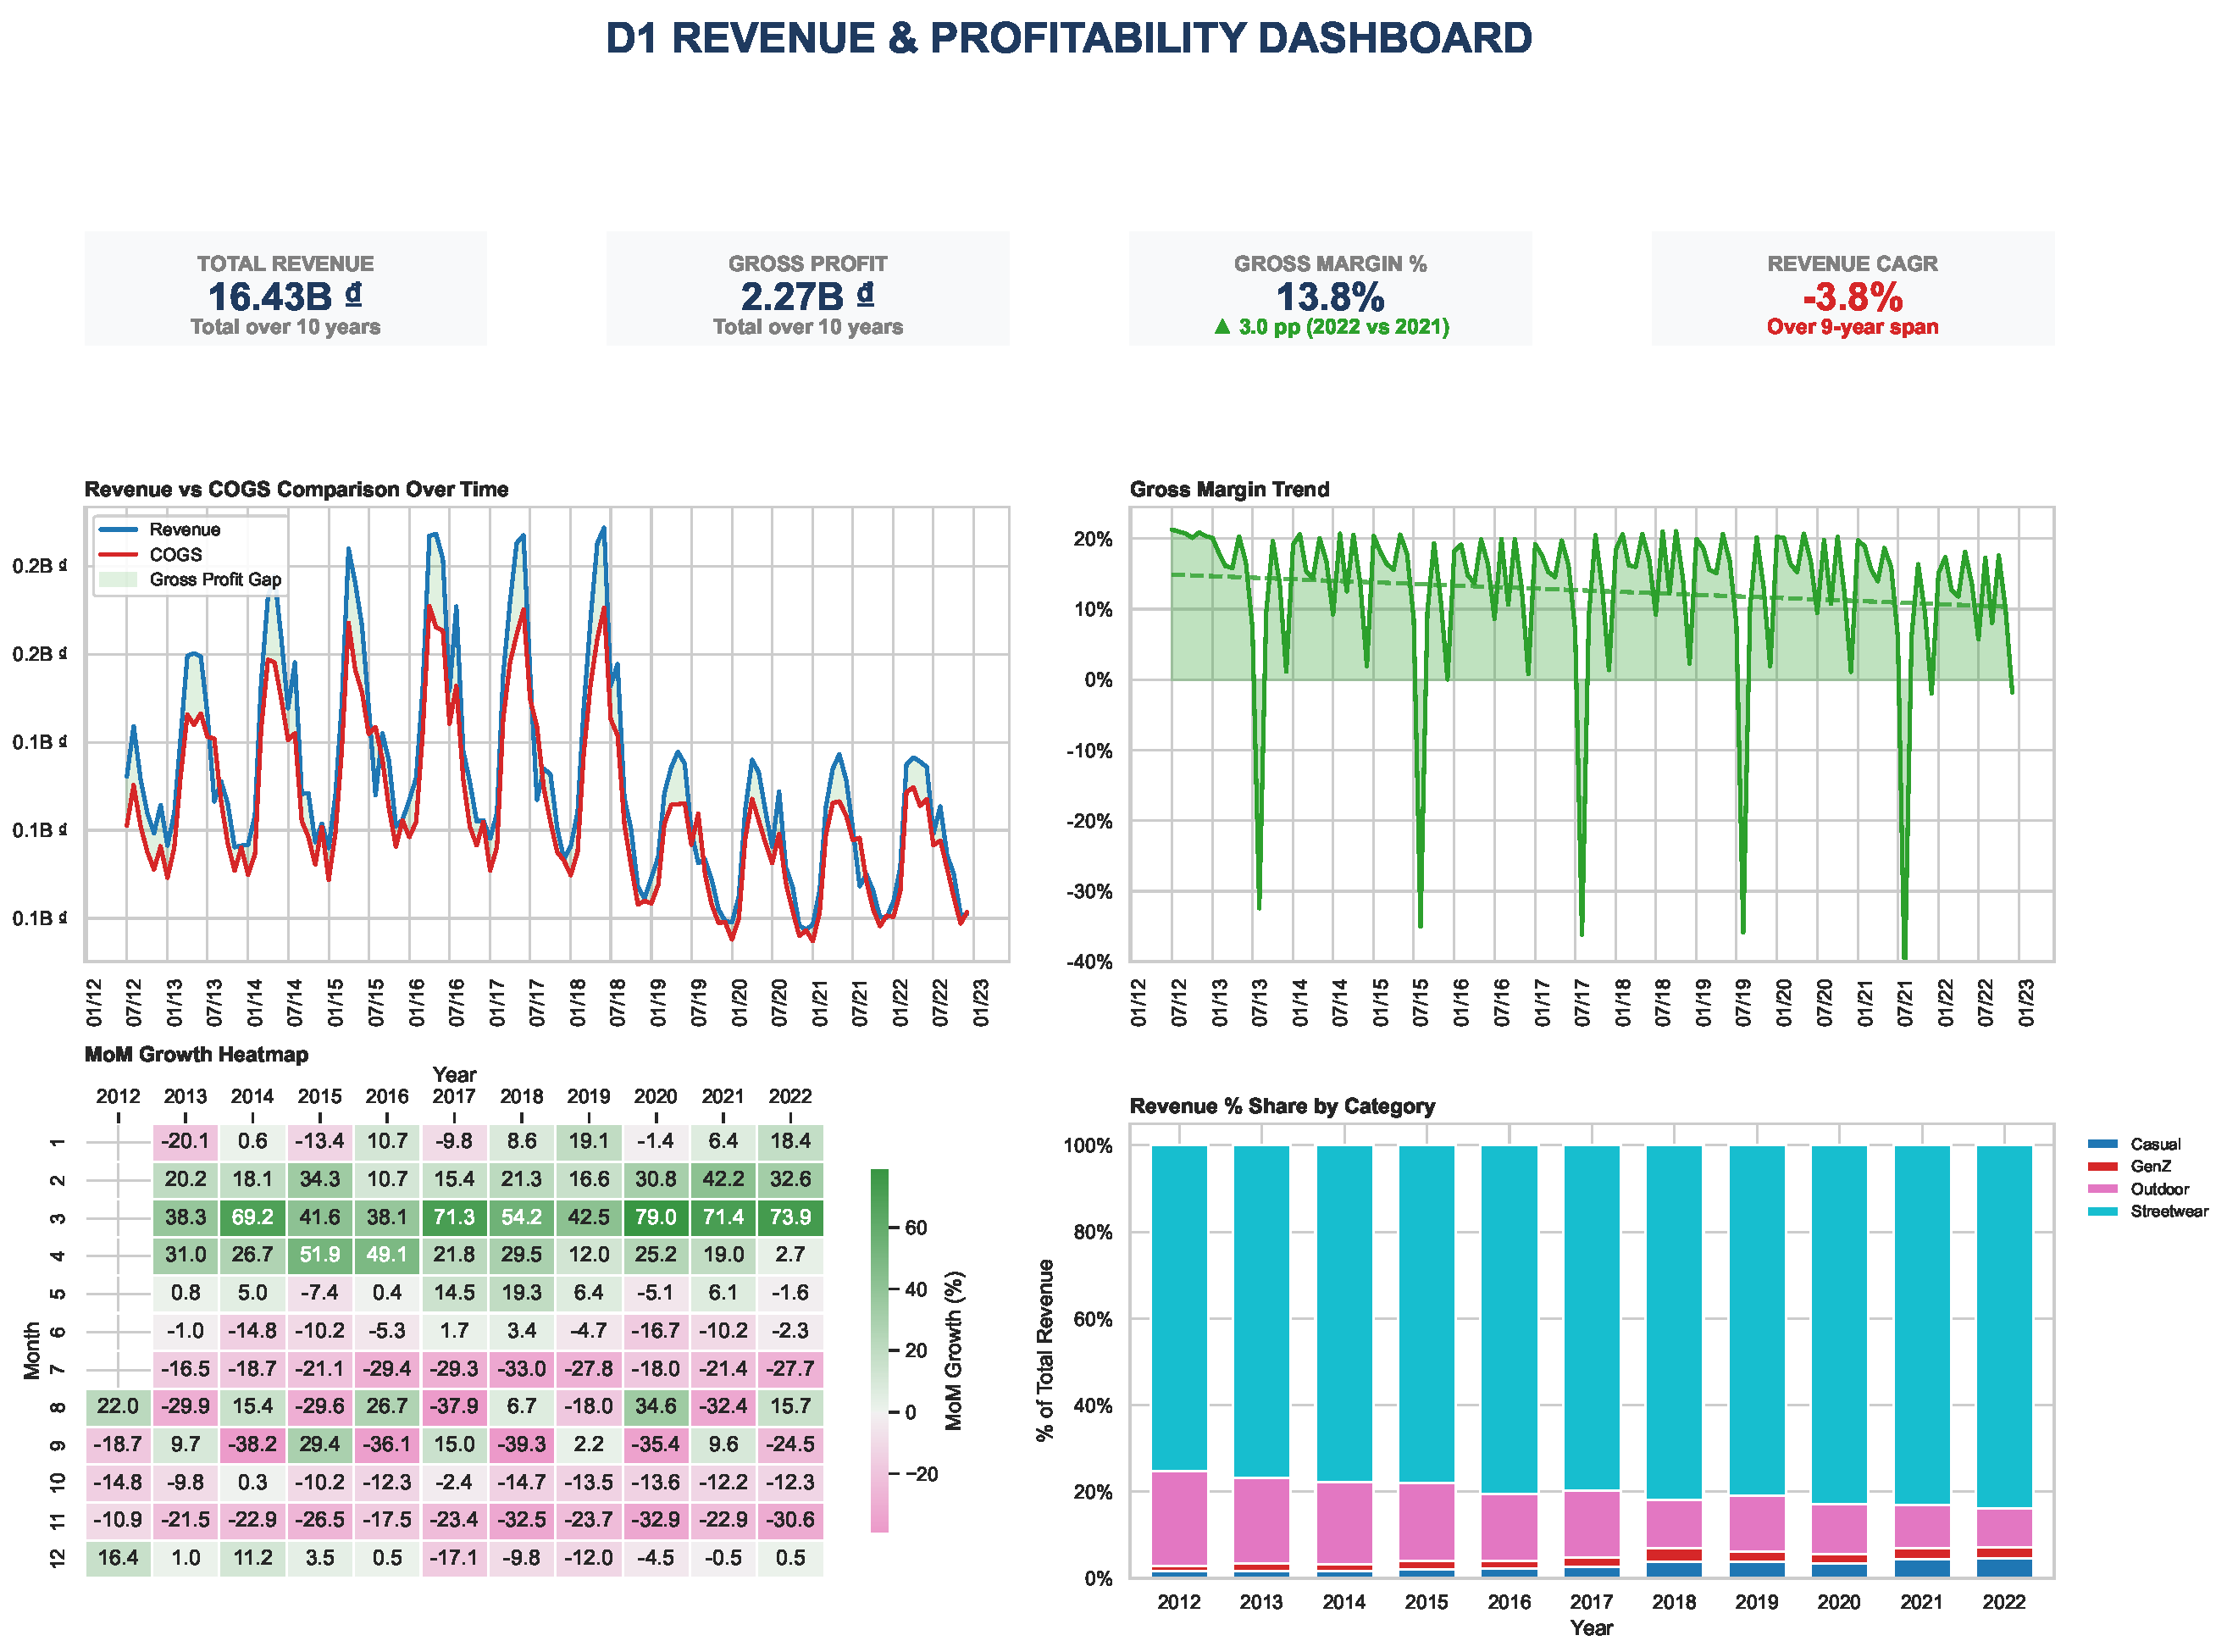
\includegraphics[width=1\textwidth]{Dashboard_D1_Static_Update.pdf}
    \caption{Tổng quan Doanh thu \& Lợi nhuận.}
    \label{fig:db1_revenue}
\end{figure}
\clearpage % Ngắt trang sau mỗi Dashboard to để tránh đè chữ

\begin{figure}[htbp]
    \centering
    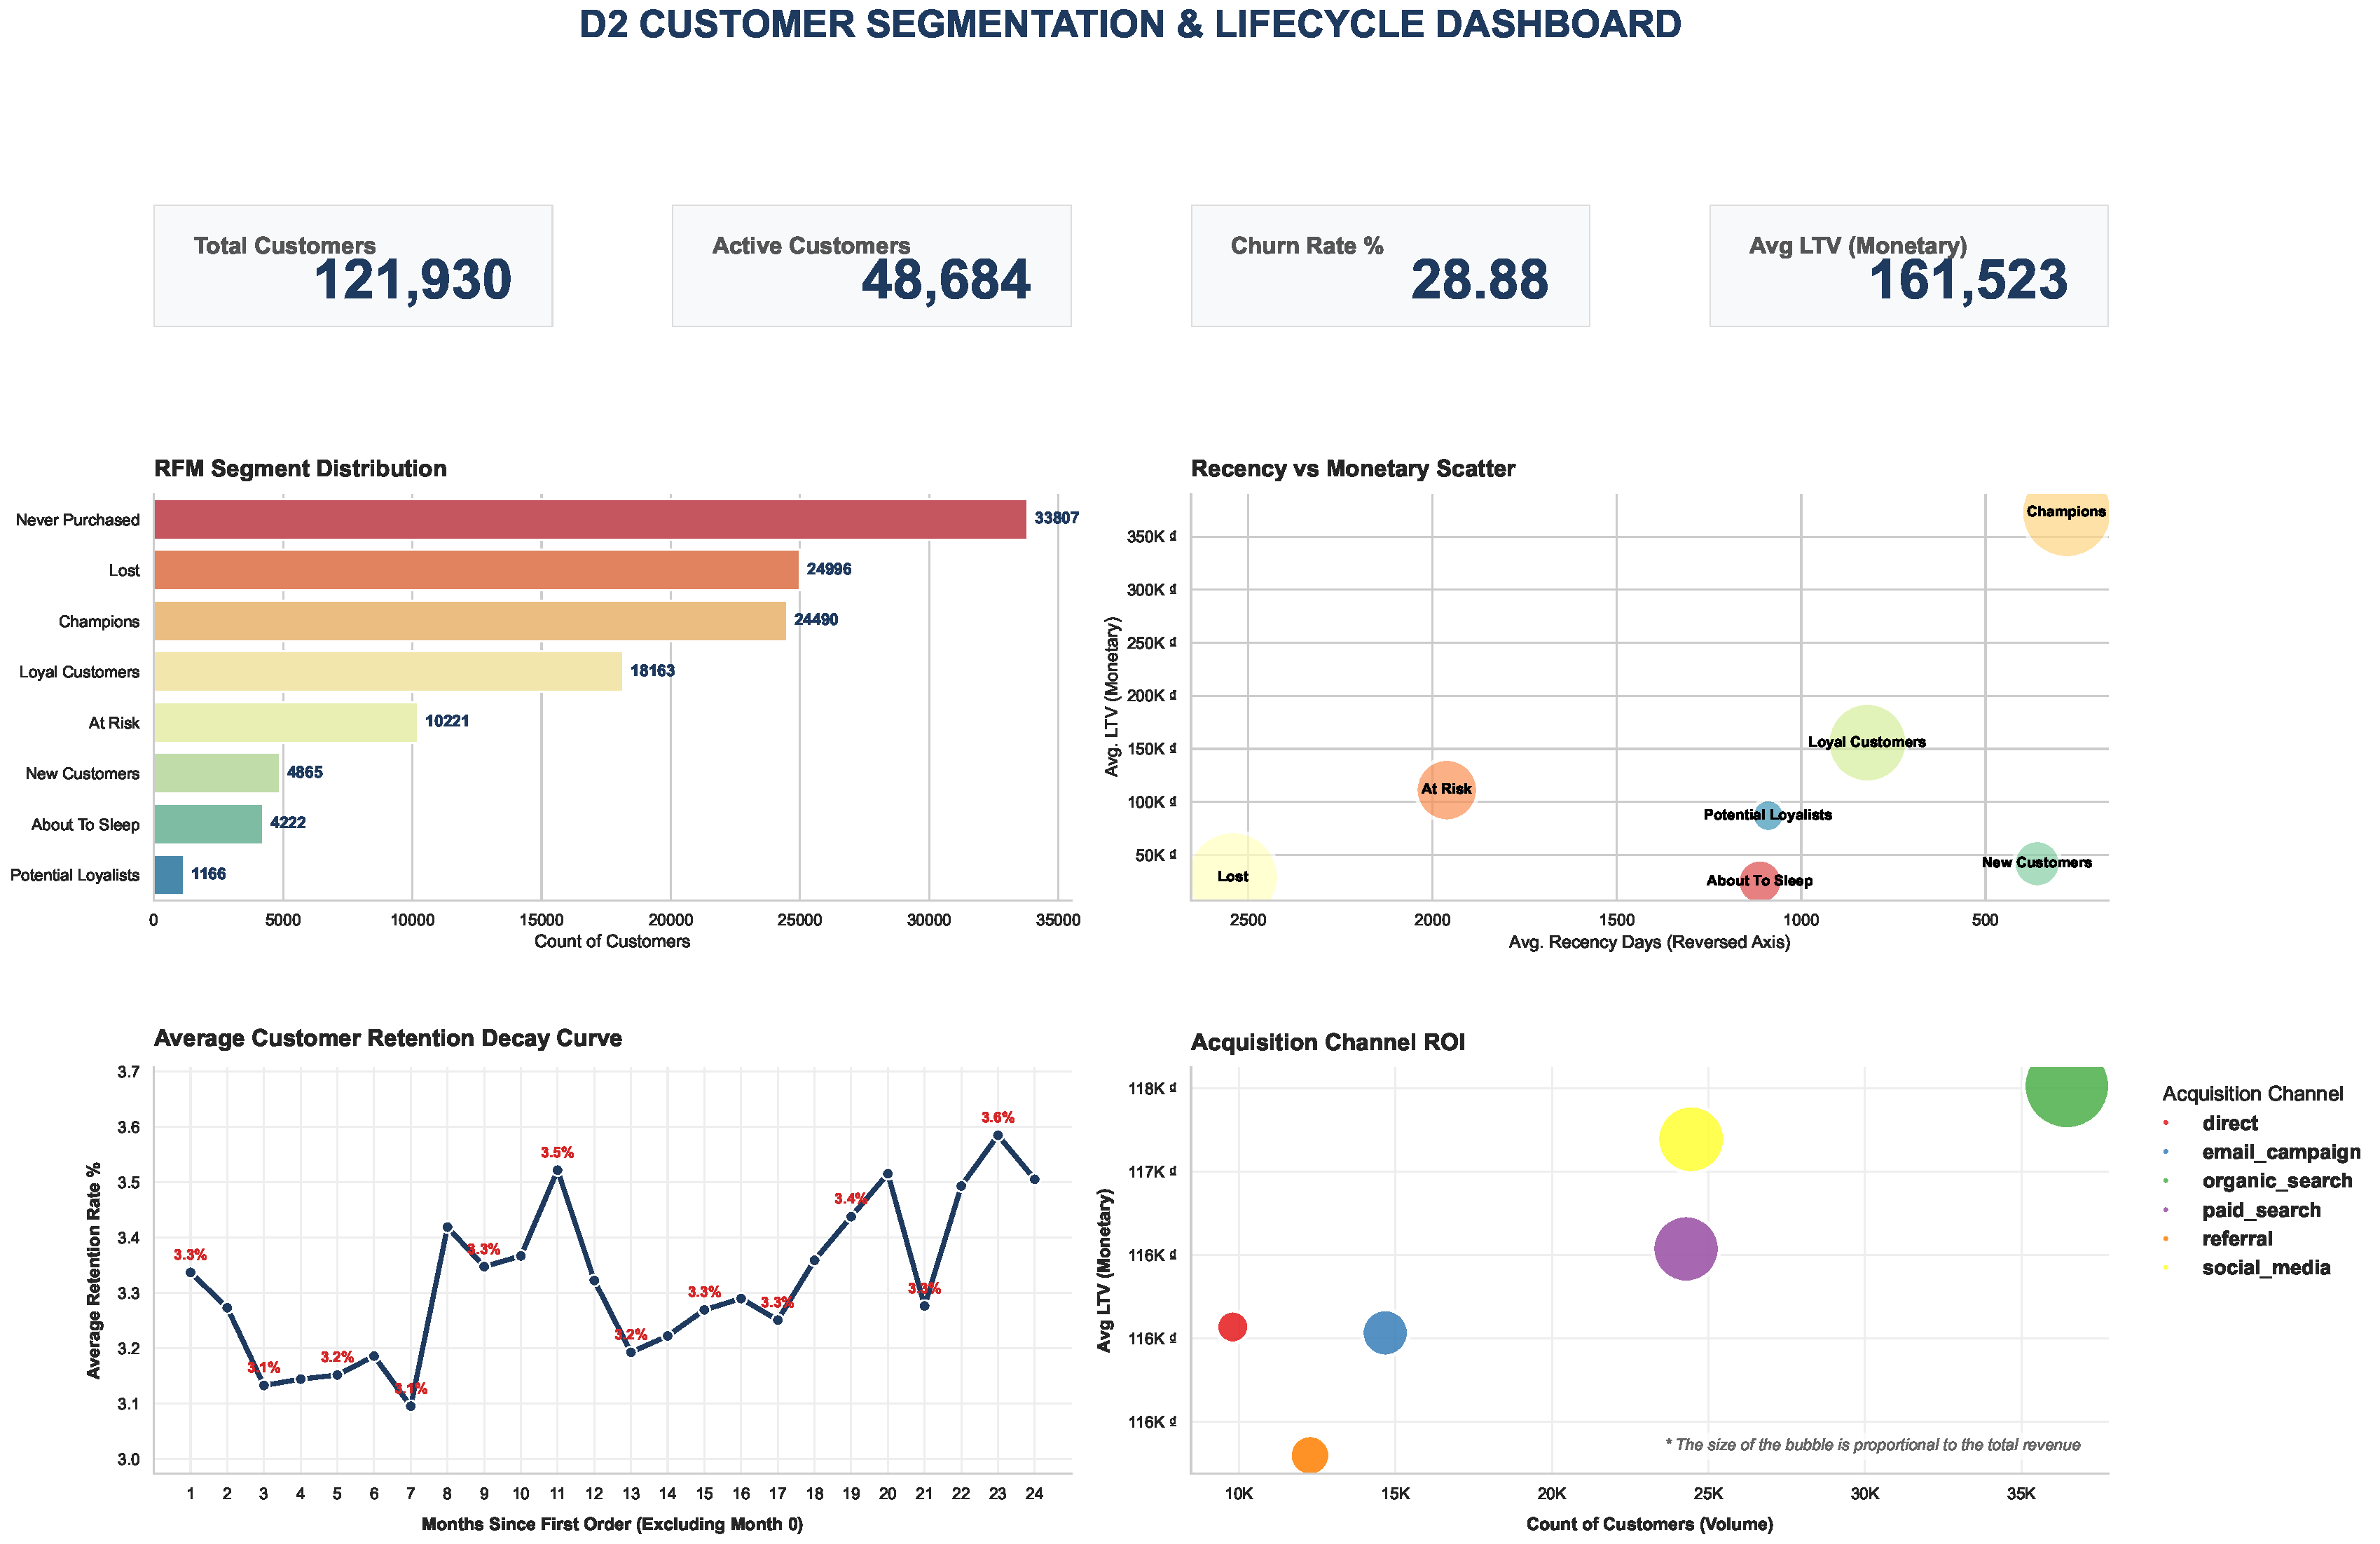
\includegraphics[width=1\textwidth]{Dashboard_D2_Final_Report_Ready.pdf}
    \caption{Phân khúc khách hàng \& Vòng đời.}
    \label{fig:db2_customer}
\end{figure}
\clearpage

\begin{figure}[htbp]
    \centering
    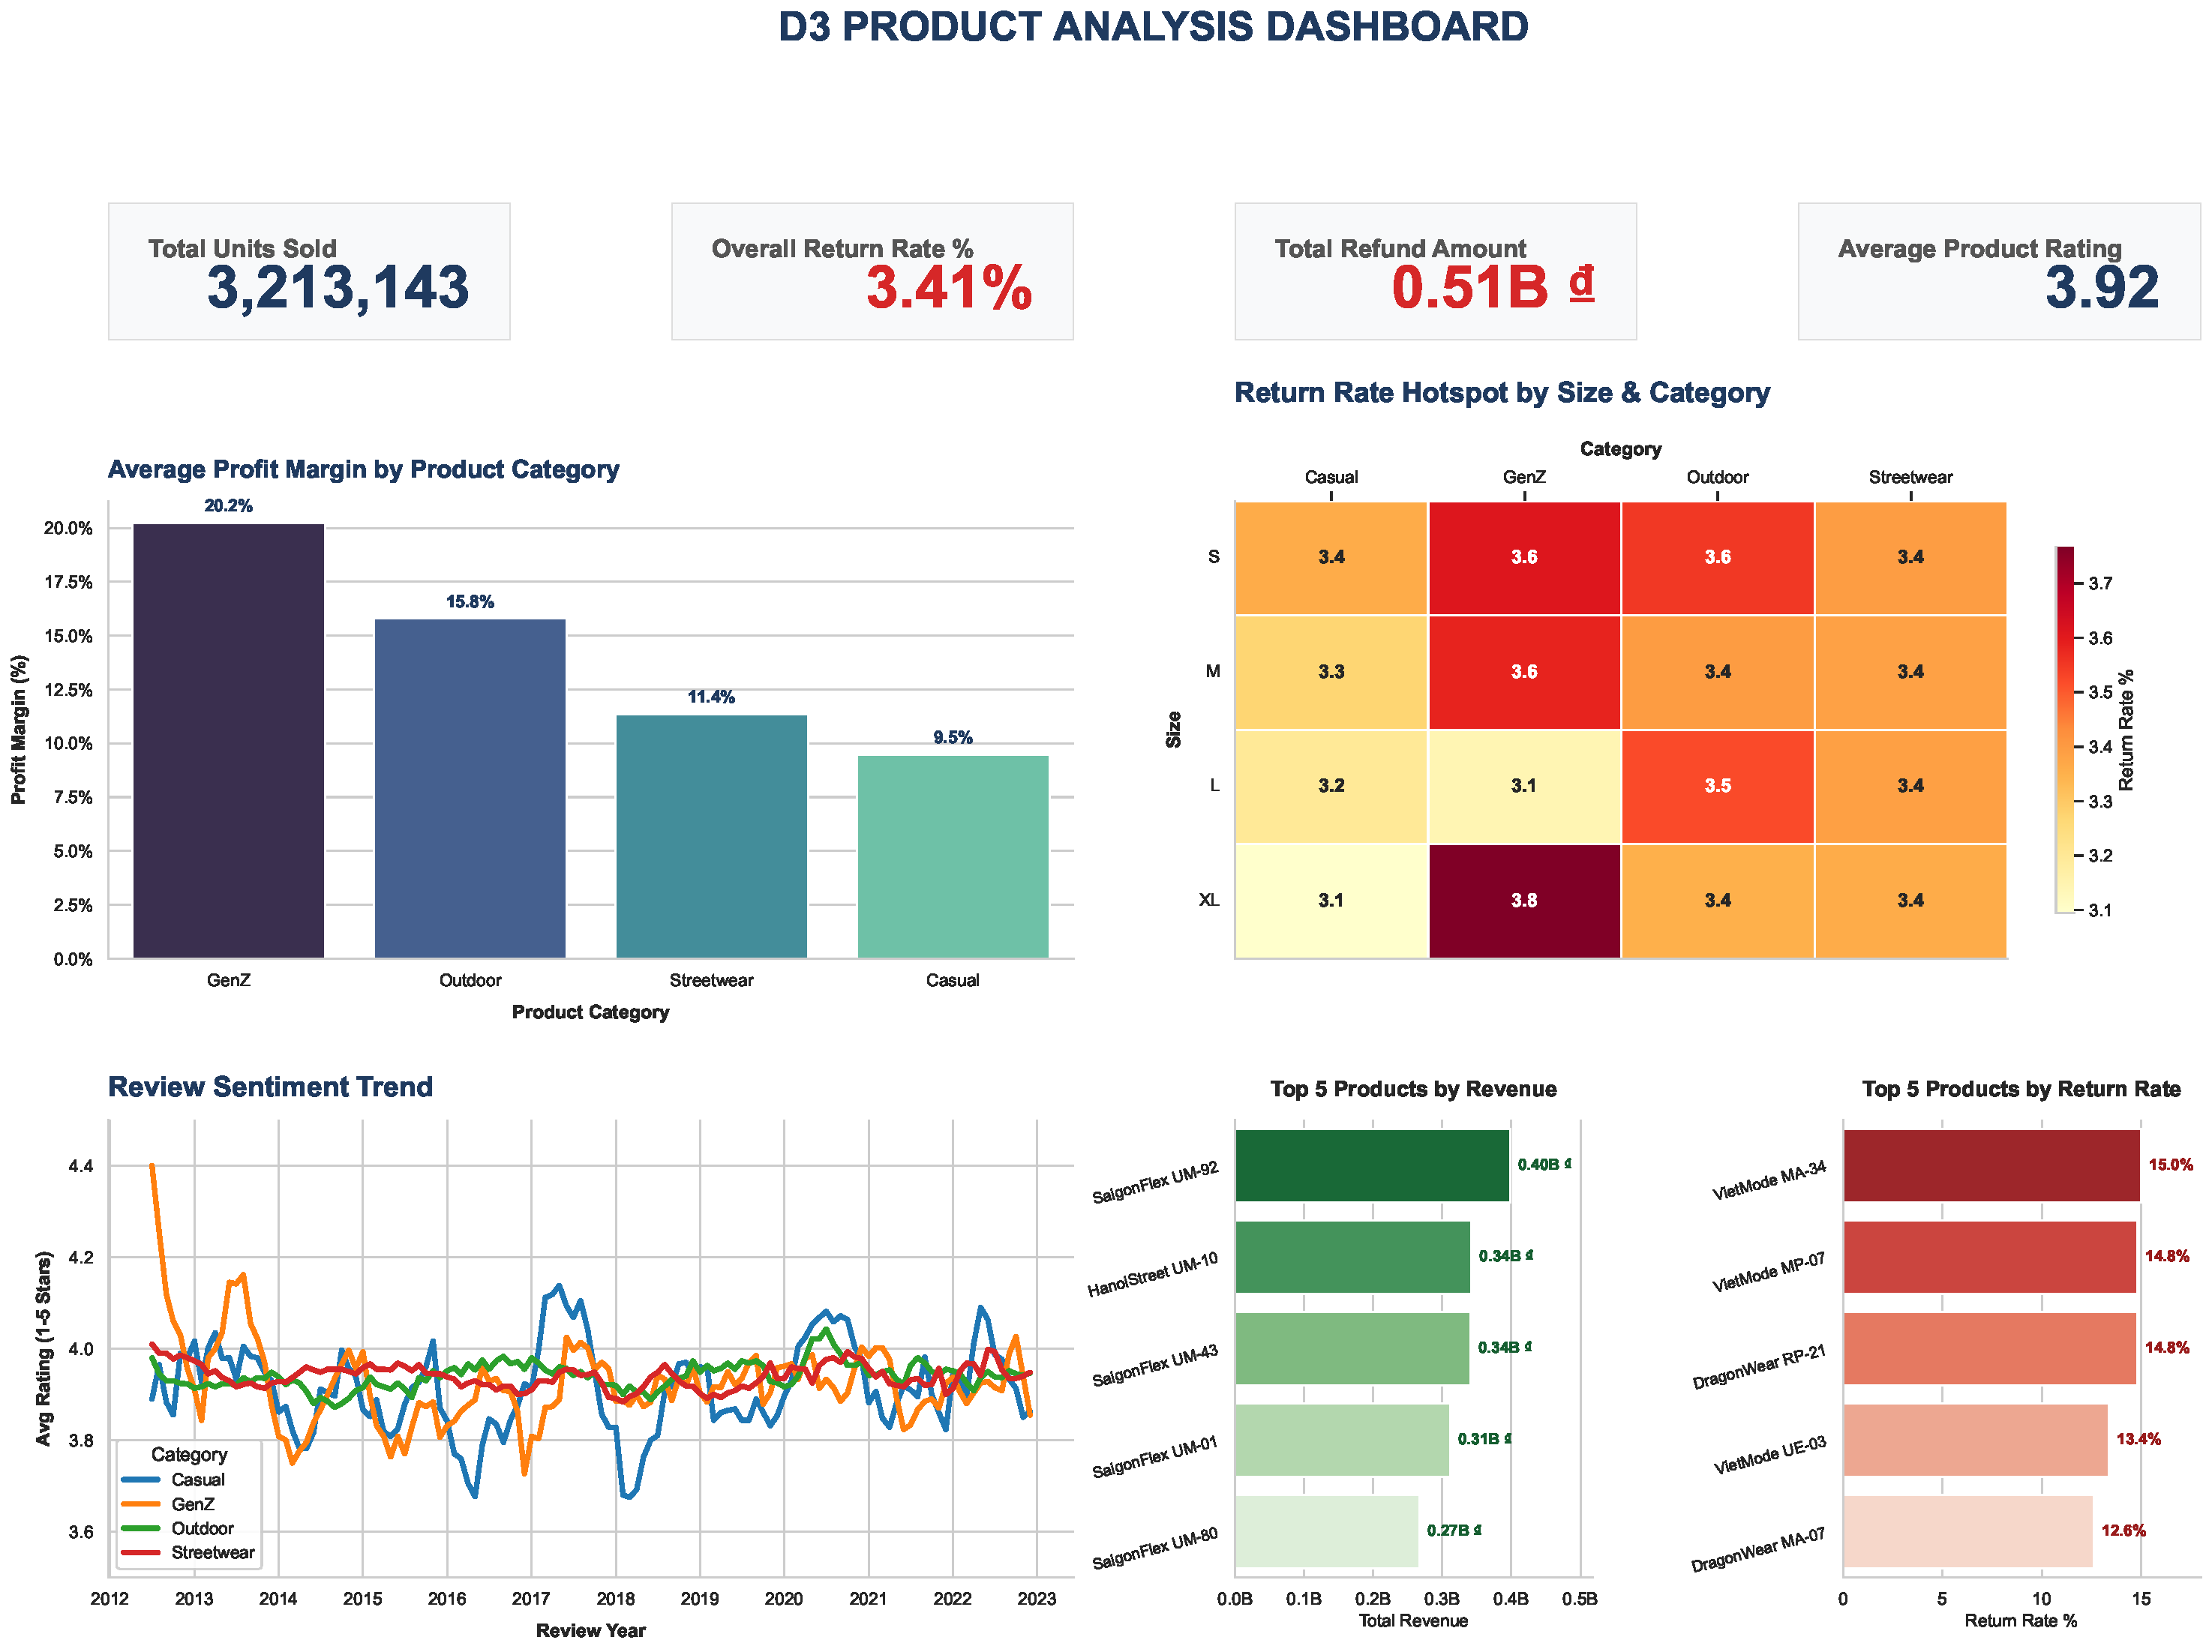
\includegraphics[width=1\textwidth]{Dashboard_D3_Final_Report_Ready.pdf}
    \caption{Phân tích sản phẩm.}
    \label{fig:db3_product}
\end{figure}
\clearpage

\begin{figure}[htbp]
    \centering
    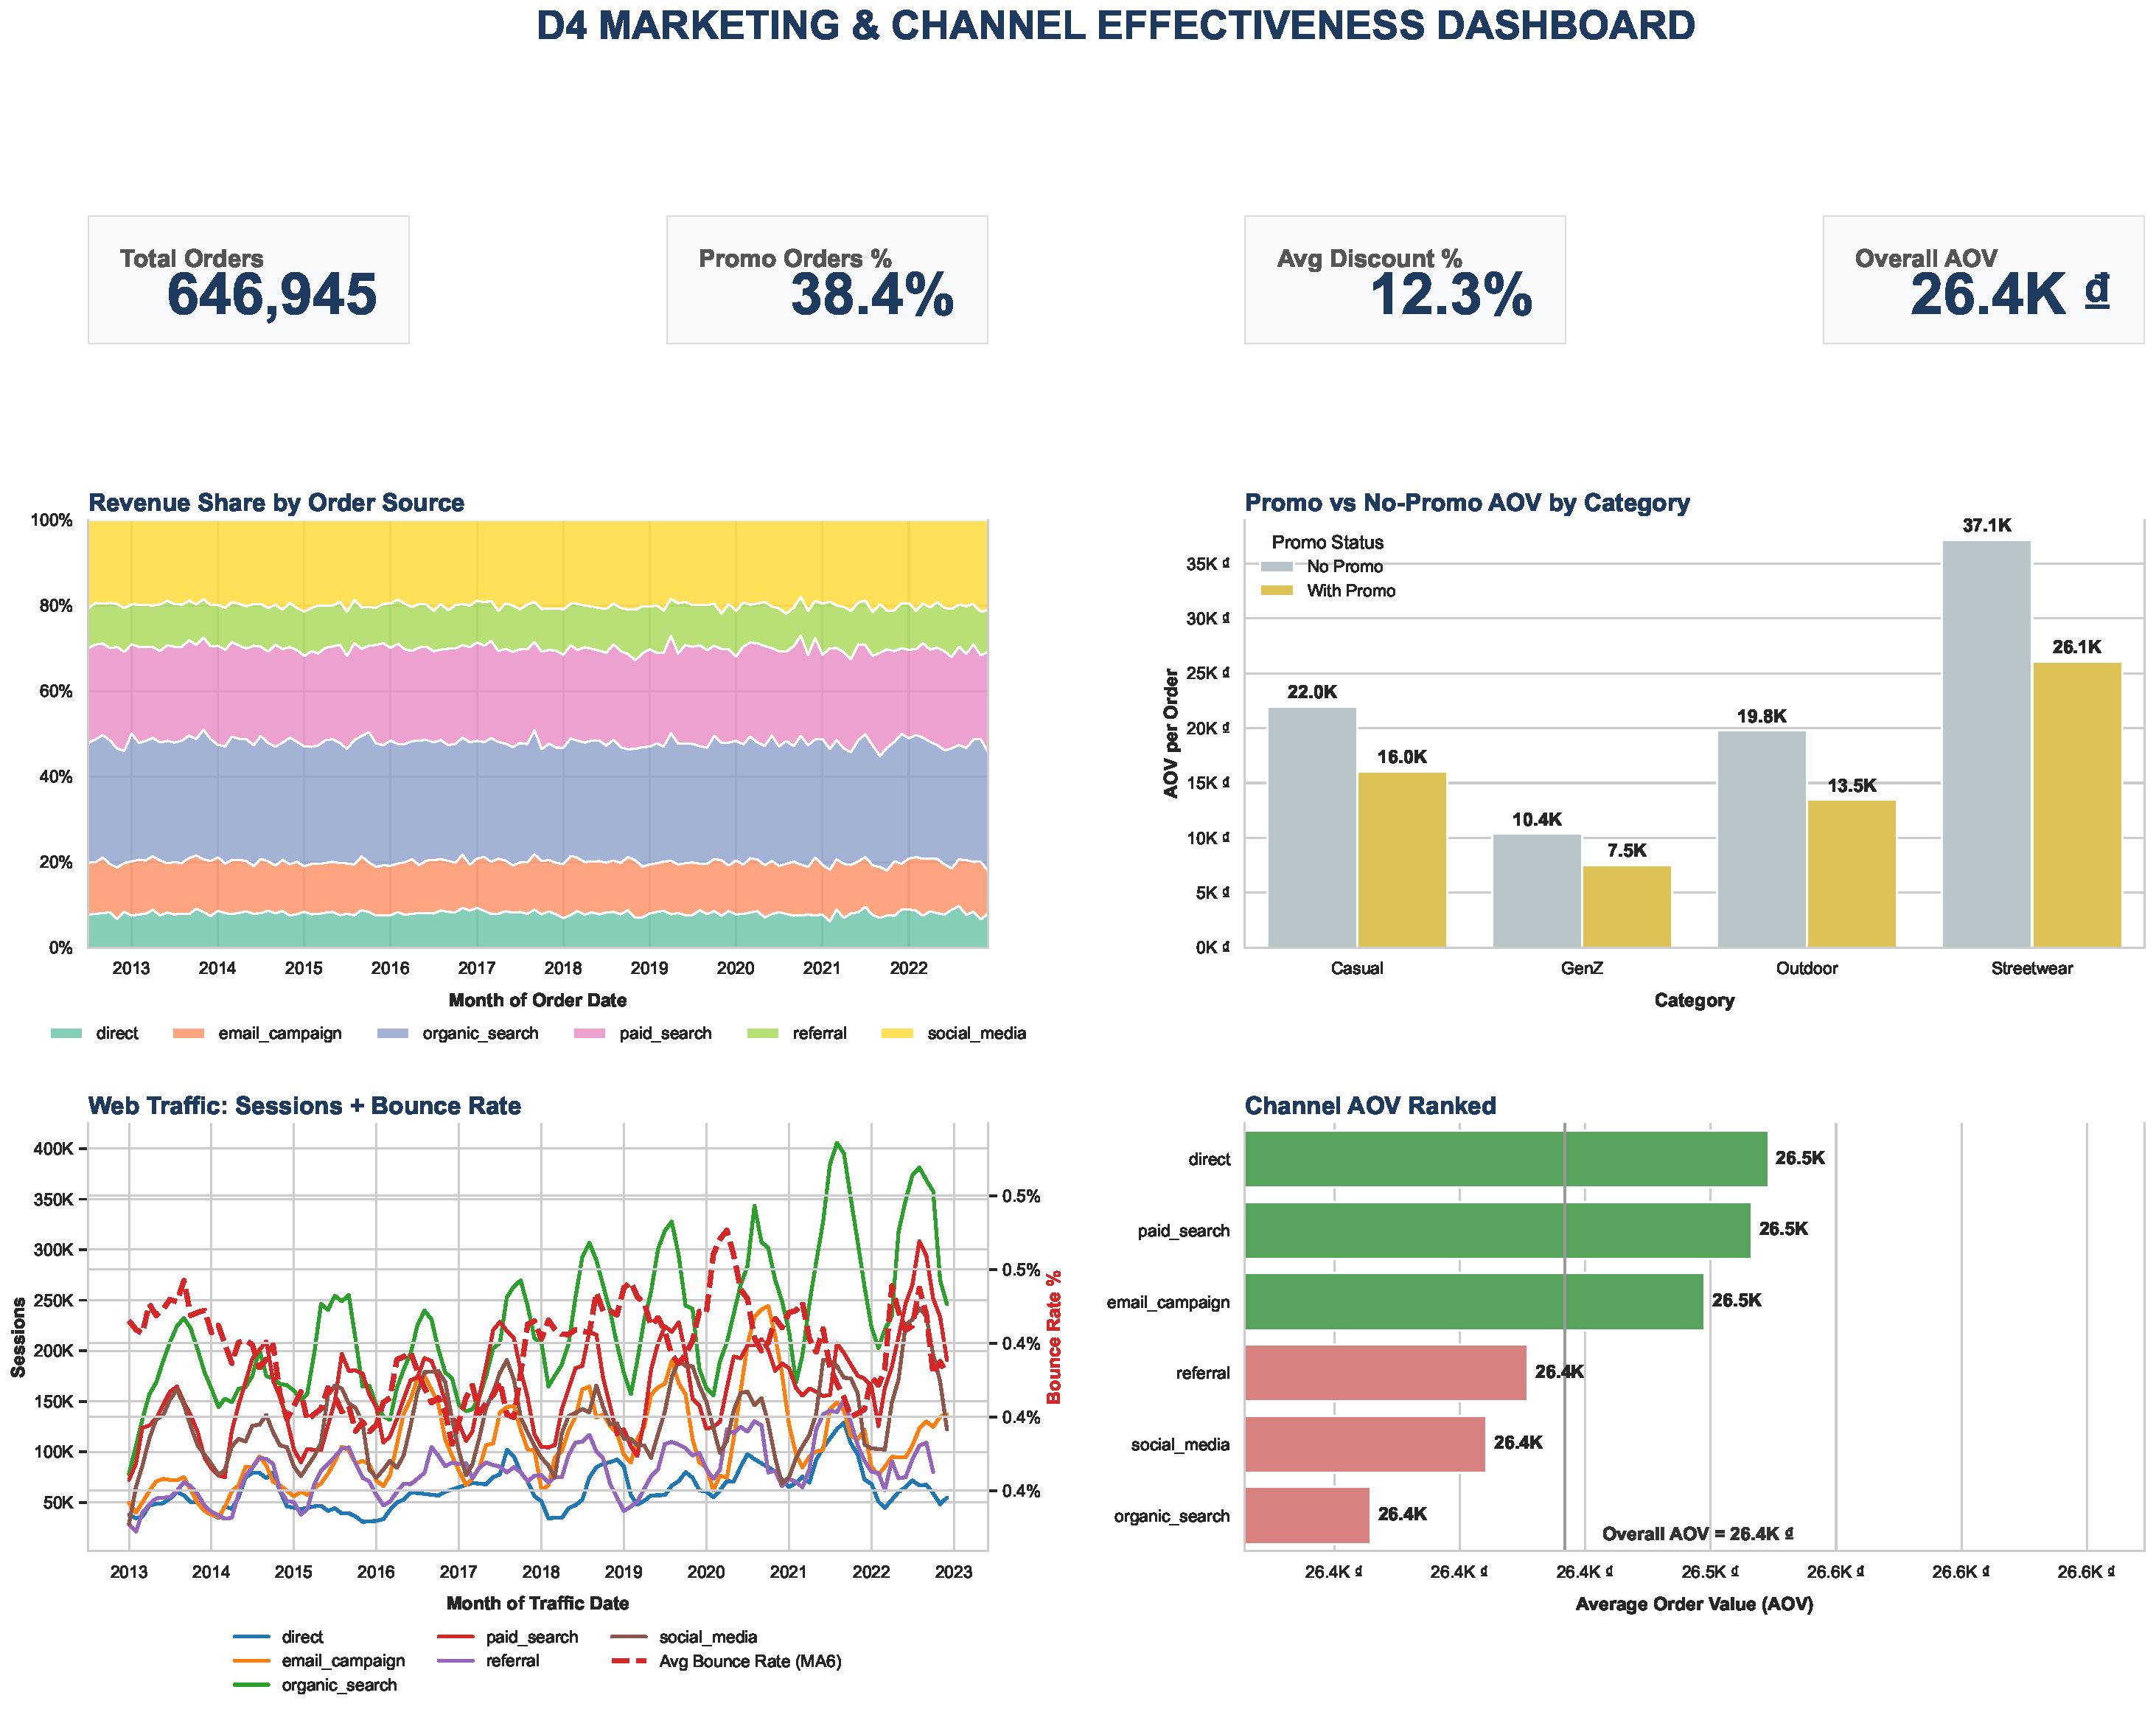
\includegraphics[width=1\textwidth]{Dashboard_D4_Final.pdf}
    \caption{Hiệu quả của các kênh truyền thông.}
    \label{fig:db4_marketing}
\end{figure}
\clearpage

\begin{figure}[htbp]
    \centering
    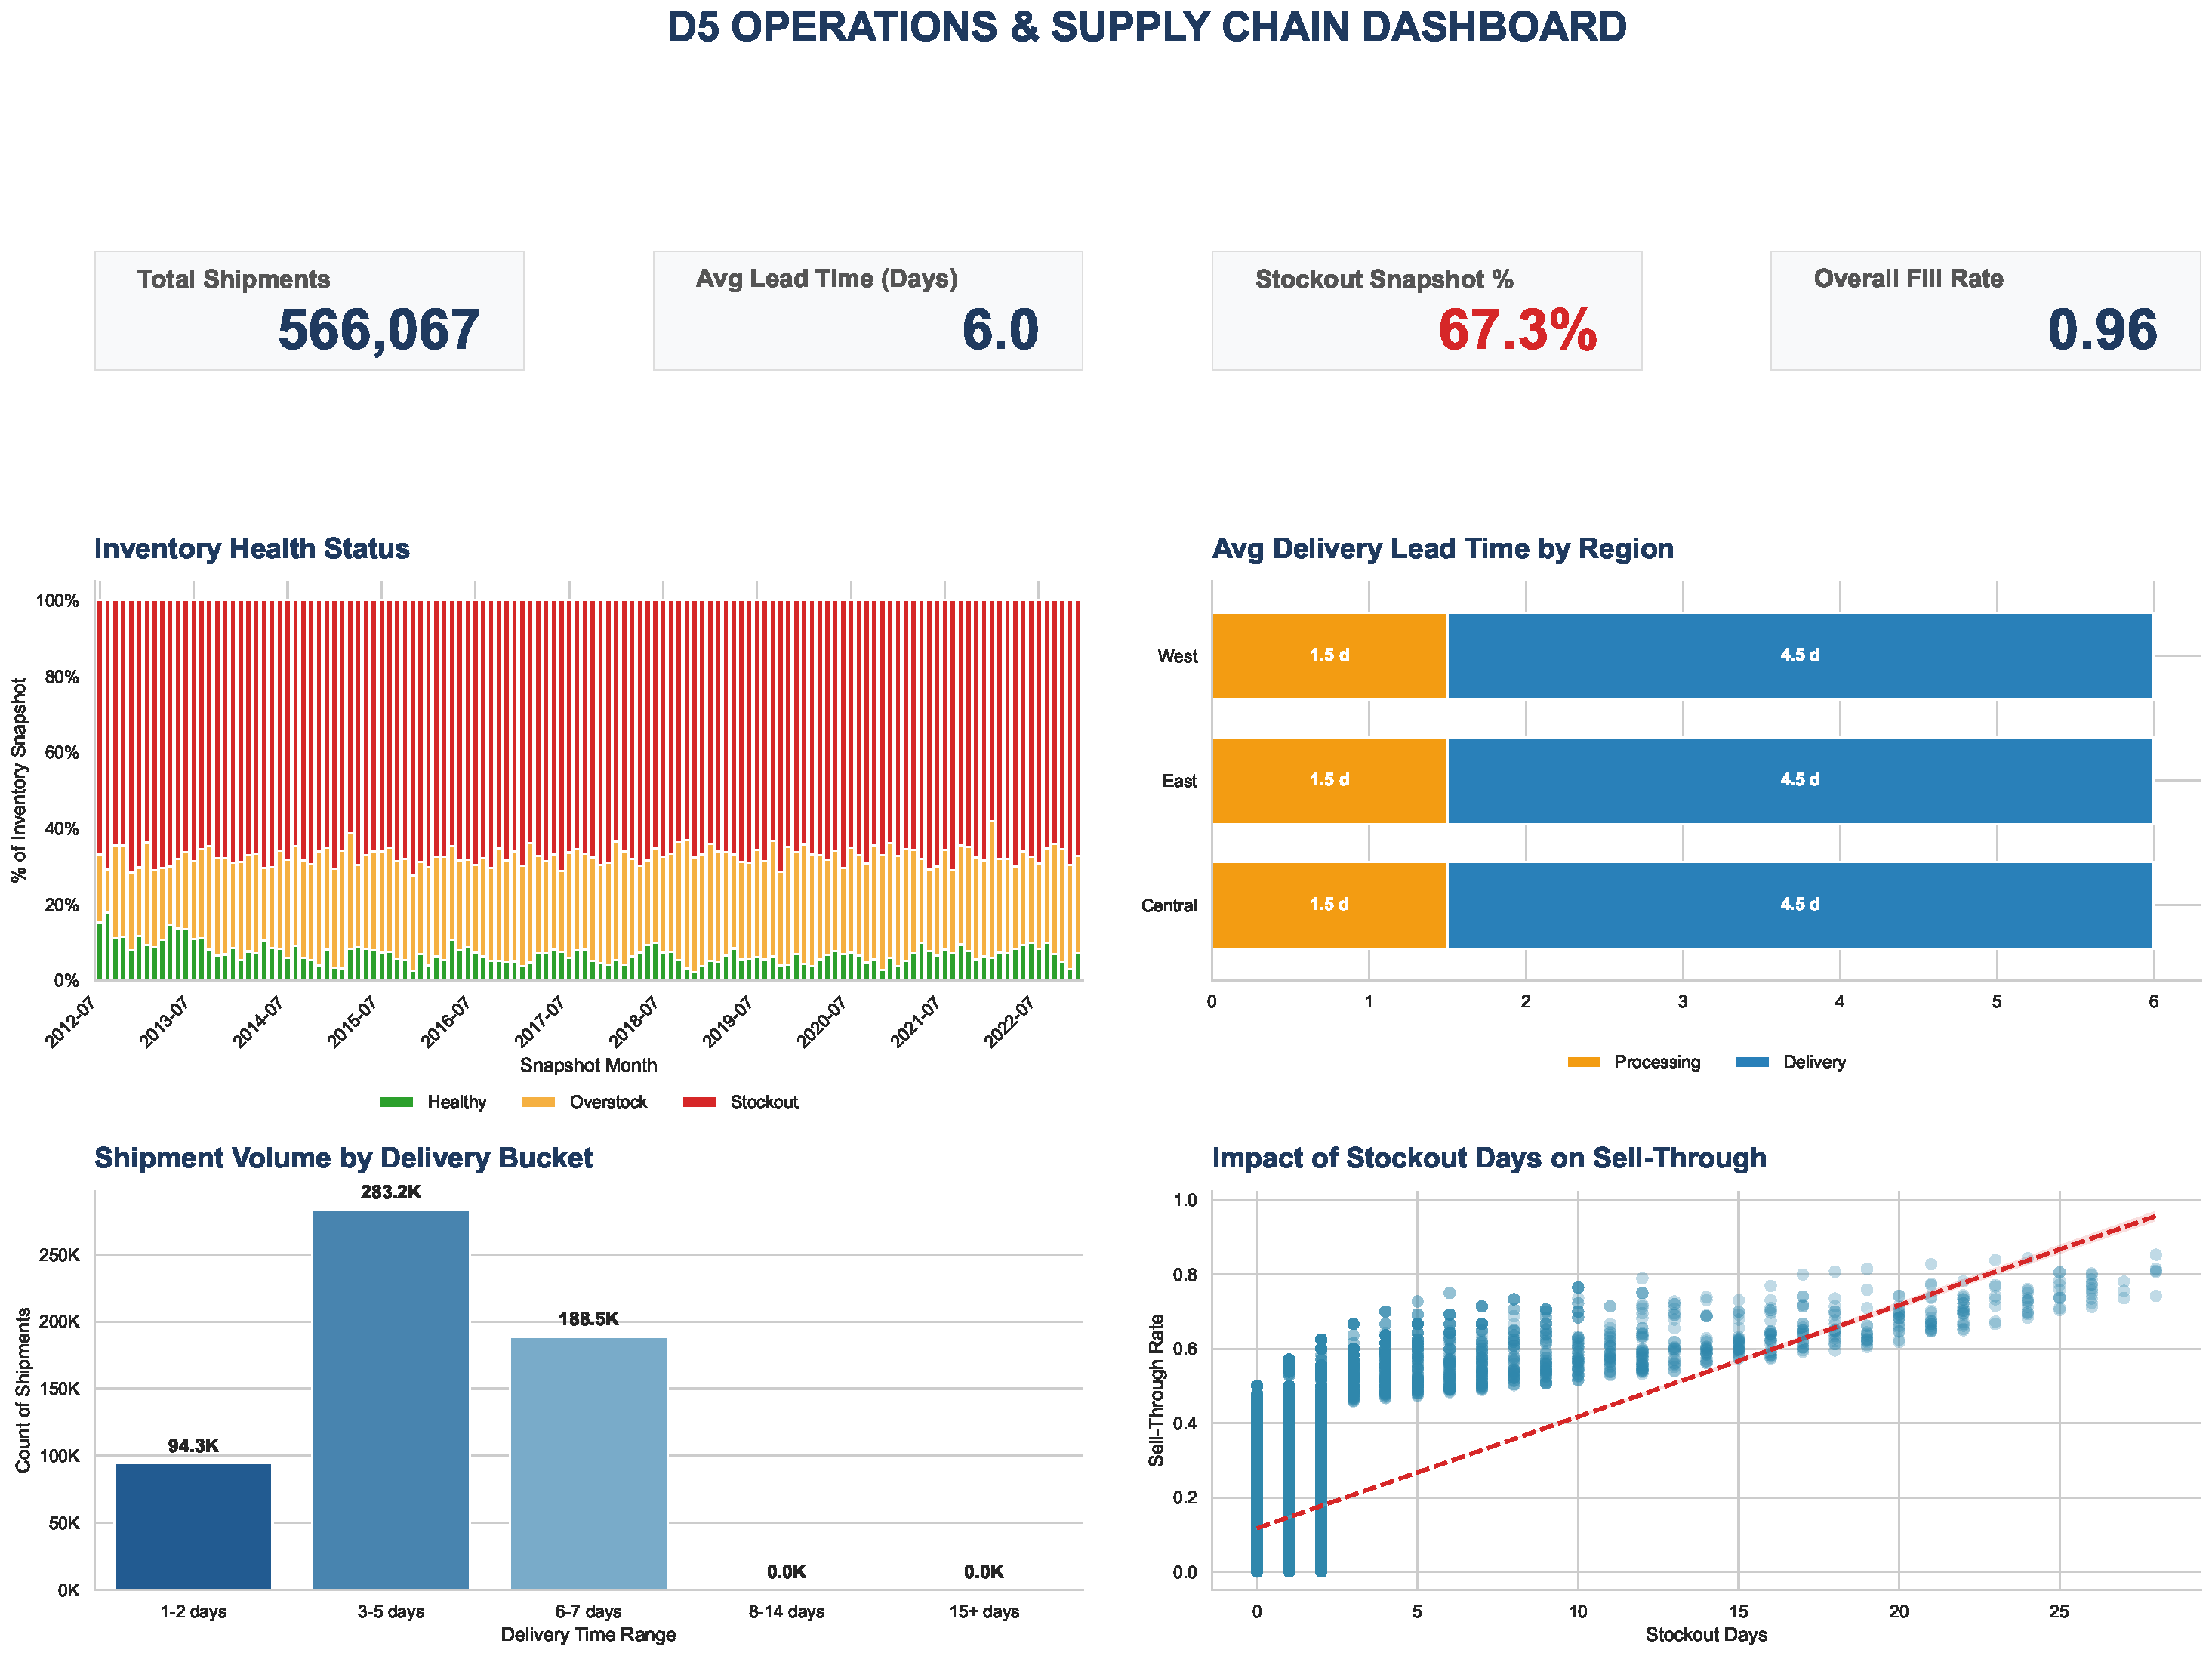
\includegraphics[width=1.2\textwidth]{Dashboard_D5_Final_Operations.pdf}
    \caption{Vận hành và chuỗi cung ứng.}
    \label{fig:db5_operation}
\end{figure}
\clearpage

% --- CÁC BIỂU ĐỒ PHỤ LỤC NHỎ HƠN (CÓ THỂ XẾP CHUNG) ---

\begin{figure}[htbp]
    \centering
    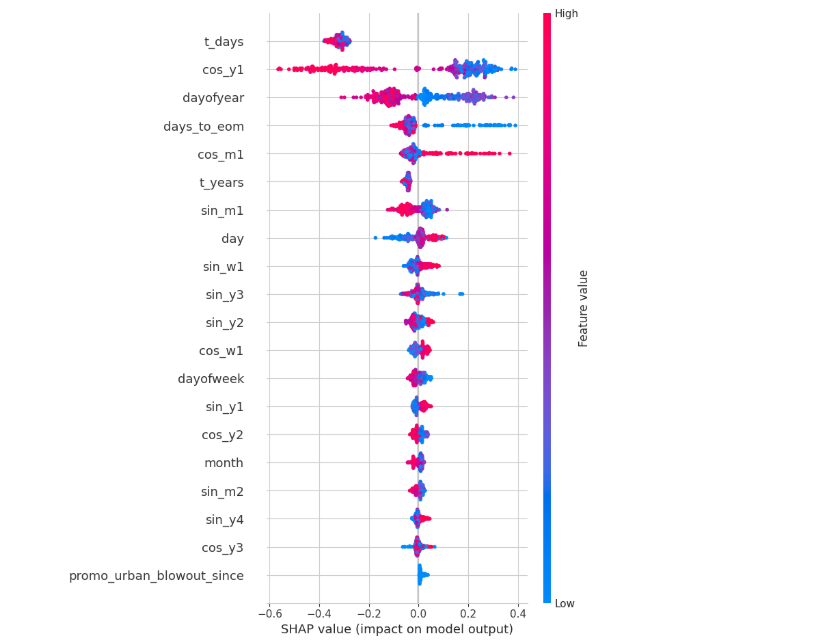
\includegraphics[width=0.85\textwidth]{SHAP_dashboard.png}
    \caption{Mức độ quan trọng của các đặc trưng thông qua phân tích SHAP Value.}
    \label{fig:shap}
\end{figure}

\vspace{1cm} % Tạo khoảng cách hở 1 chút giữa 2 biểu đồ

\begin{figure}[htbp]
    \centering
    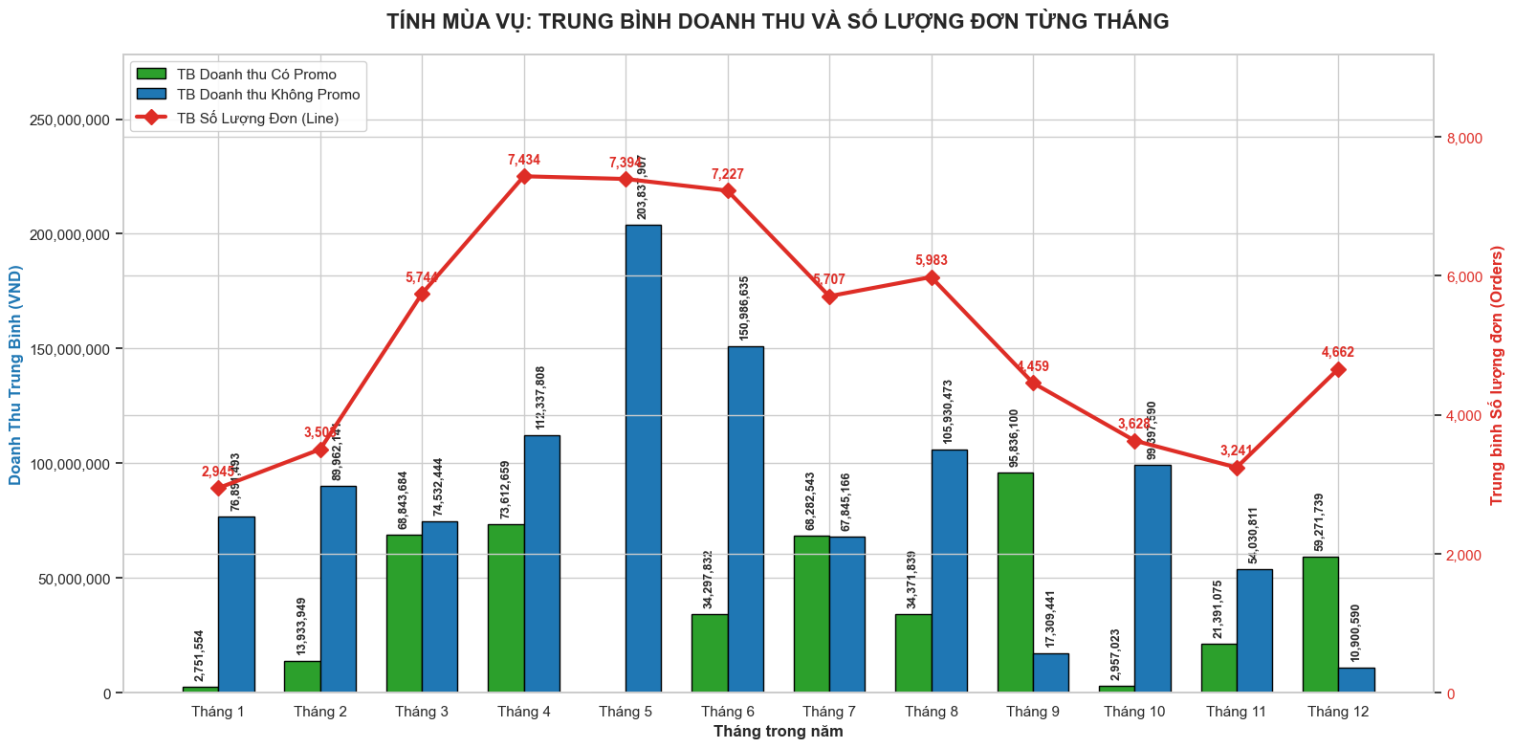
\includegraphics[width=0.85\textwidth]{D6_promo.png}
    \caption{Trung bình doanh thu và số lượng đơn theo từng tháng.}
    \label{fig:d6_promo} % ĐÃ SỬA LỖI TRÙNG LABEL
\end{figure}
\clearpage

\begin{figure}[htbp]
    \centering
    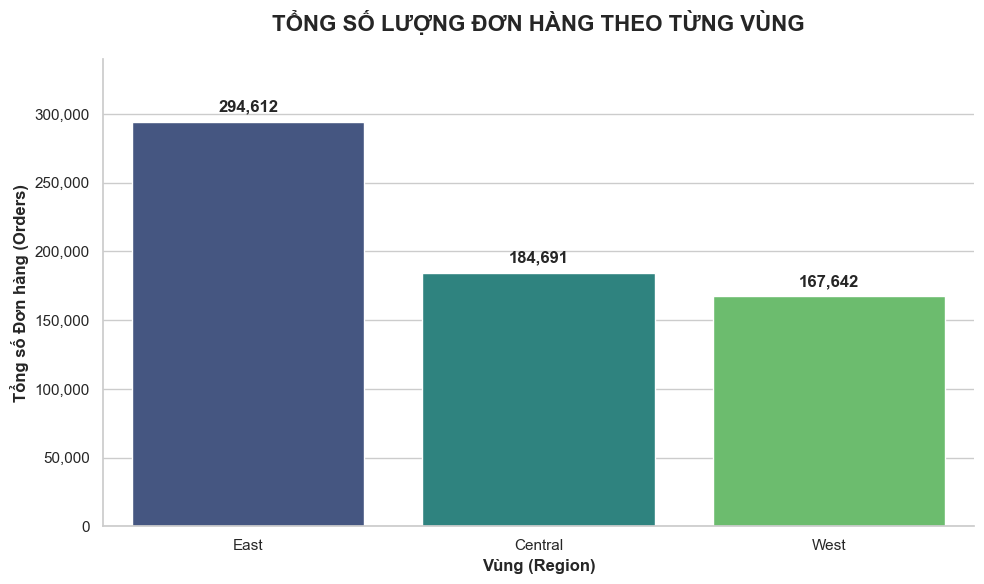
\includegraphics[width=0.85\textwidth]{D7_Area.png}
    \caption{Tổng số lượng đơn hàng theo từng vùng.}
    \label{fig:d7_area} % ĐÃ SỬA LỖI TRÙNG LABEL
\end{figure}

\end{document}